\section{Datenbeschreibung}
\label{sec:Datenbeschreibung}

Der vorliegende Datensatz besteht aus insgesamt 949 Bildern von Autos mit
Nummernschildern.\footnote{Die Originaldaten sind unter \url{https://github.com/phibuc/Lab_FS_Data},
    sowie unter \url{https://github.com/RobertLucian/license-plate-dataset}
    einsehbar.}
Die Bilder wurden in den Regionen Brasilien, Europa, Rum\"anien und USA
aufgenommen.

Zu jedem Bild liegen au{\ss}erdem Informationen zur Position
des Nummernschildes innerhalb des Bildes anhand von Pixel Koordinaten vor.
Die Position des Nummernschildes ist dabei durch die Koordinaten
$x_{\text{min}}$, $x_{\text{max}}$, $y_{\text{min}}$, $y_{\text{max}}$
relativ zur linken oberen Ecke des Bildes eindeutig spezifiziert.

In Abbildung~\ref{fig:autos} sind drei Beispielbilder aus dem Datensatz
dargestellt. Die Koordinaten der Nummernschilder sind anhand der
roten Rechtecke eingezeichnet.

\begin{figure}[h]
    \centering
    \begin{subfigure}{0.32\textwidth}
        \centering
        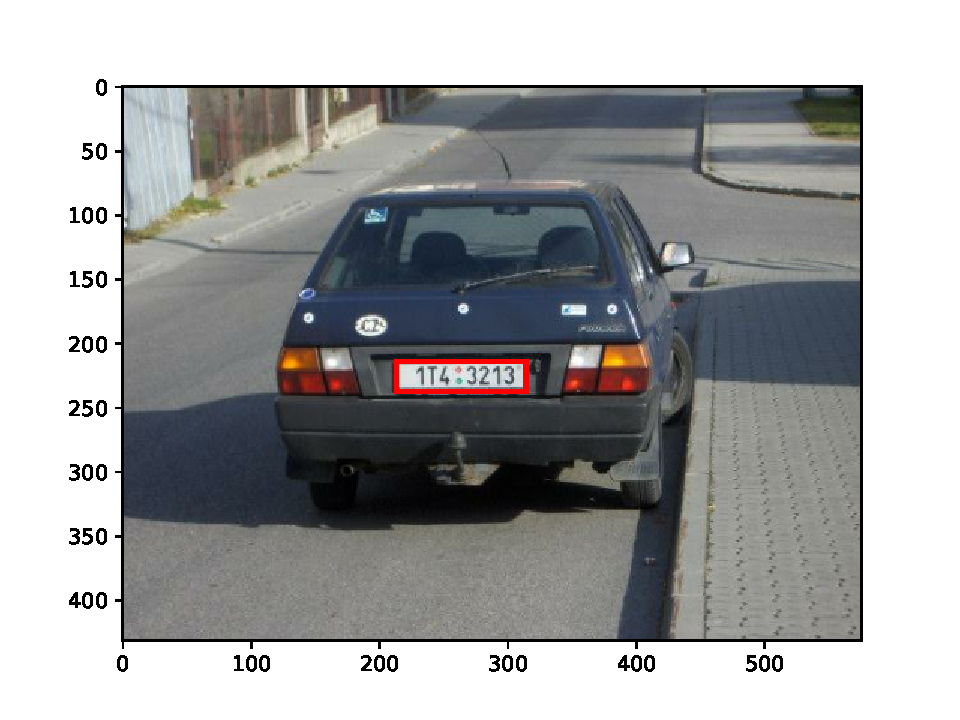
\includegraphics[width=\textwidth]{abbildungen/car_1}
    \end{subfigure}
    \begin{subfigure}{0.32\textwidth}
        \centering
        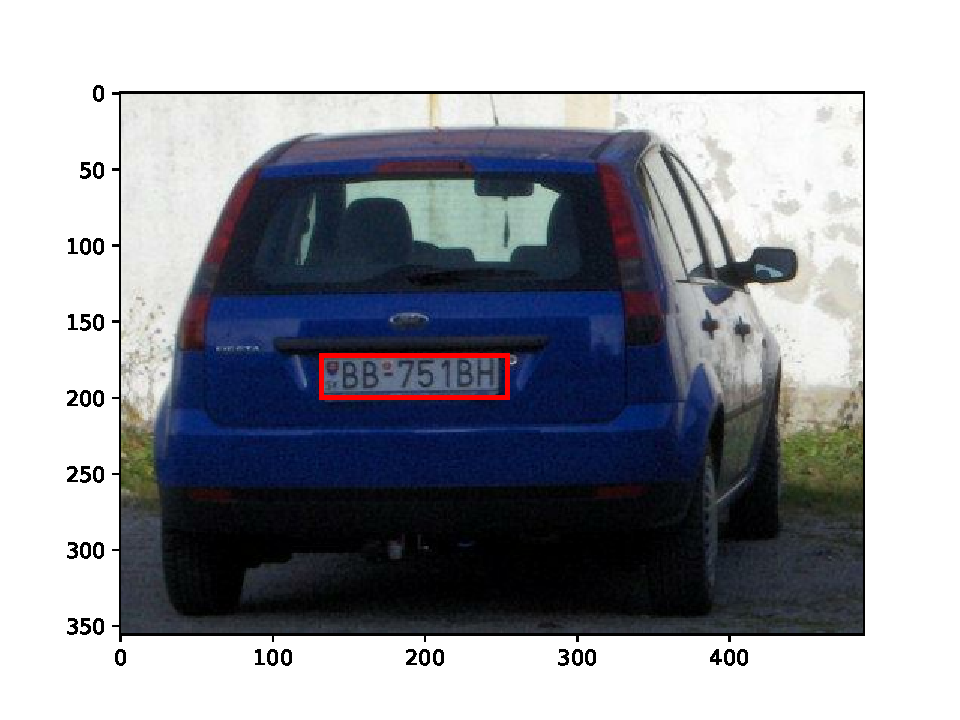
\includegraphics[width=\textwidth]{abbildungen/car_2}
    \end{subfigure}
    \begin{subfigure}{0.32\textwidth}
        \centering
        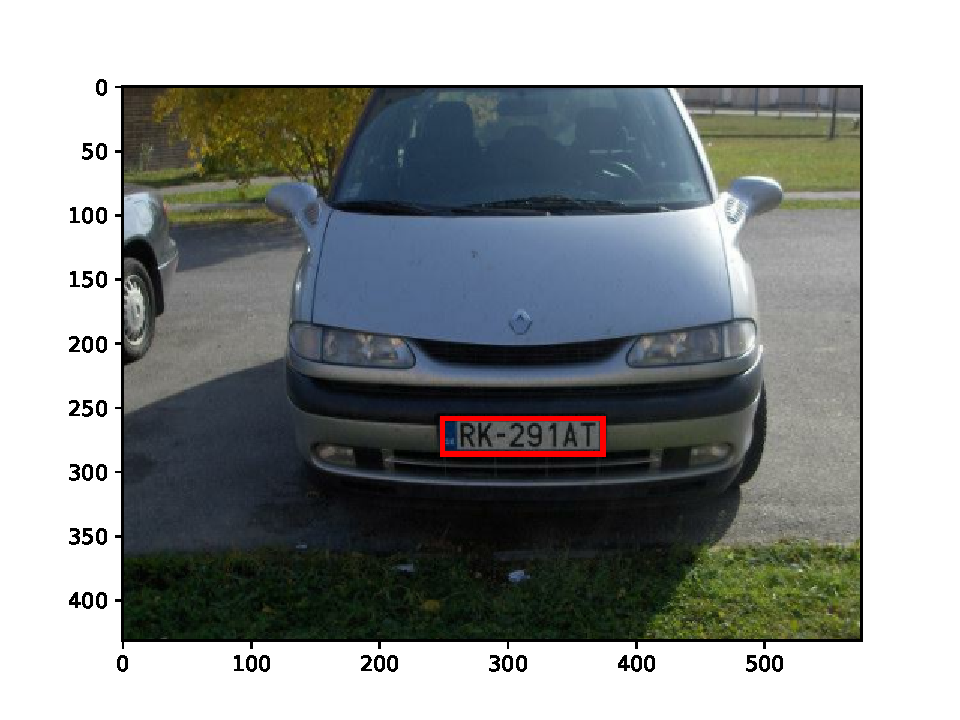
\includegraphics[width=\textwidth]{abbildungen/car_3}
    \end{subfigure}
    \caption{Drei Beispiele aus dem vorliegenden Datensatz.
        Die Nummernschilder sind anhand ihrer Koordinaten rot umrandet.}
    \label{fig:autos}
\end{figure}